%%% Thesis Introduction --------------------------------------------------
\chapter{Introduction}

\graphicspath{ {Introduction/IntroductionFigs/PNG/}
  {Introduction/IntroductionFigs/PDF/}
  {Introduction/IntroductionFigs/} }

La modélisation géométrique a permis, dans un premier temps, de
représenter des modèles virtuels. De ce fait, des outils permettant la
modification de ces modèles se sont directement mis en place, au
travers du déplacement des différents sommets des modèles. Les
déformations engendrées étaient liées à la représentation interne de
l'objet. Mais d'autres types de déformation se sont instaurées par la
suite, comme la déformation \textit{spatiale}.
\\

La déformation spatiale consiste à déformer un objet en modifiant son
espace ambiant.  On notera \cite{Bar84} et \cite{SP86} comme étant les
premiers à avoir introduit ce type de déformation. Ce procédé a un
avantage considérable, la modification de l'espace. En effet comme la
déformation est réalisée sur chaque point de l'espace de façon
indépendante, elle n'est pas liée à la représentation interne de
l'objet. Cette propriété est essentielle, car elle permet d'assurer
que, peu importe la topologie existante entre les points de l'espace à
déformer, une même déformation de l'outil déformera l'espace de la
même manière.
\\

La première partie de ce travail consiste en la réalisation d'un
mélange de multiples outils de déformation. En parallèle, une étude
est faite sur les outils de déformation de différentes dimensions,
pour déterminer le meilleur outil associé à chaque dimension (point,
courbe, surface, volume). Au final il s'agira de pouvoir obtenir une
génération automatique d'un outil multidimensionnel de déformation
associé à un modèle, en segmentant ce dernier et en associant à
chacune de ses segmentations l'outil de déformation le plus adapté à
sa forme.
\\

On voudrait, pour un même modèle, associer des outils bien précis à
certaines parties de ce modèle. Prenons le modèle de l'alligator
(Figure \ref{INTall}), on voudrait ouvrir la bouche de l'alligator,
élargir son ventre et bouger sa queue, mais ce n'est pas possible avec
un seul outil. L'idée serait alors d'appliquer des outils différents
(ou des outils de résolutions différentes) sur différentes zones d'un
objet, ou plusieurs outils sur une même zone. On se demande alors
comment mélanger ces outils de façon à ce que les déformations se
fassent de manière continue.
\\

De plus, en fonction de la précision de la déformation à appliquer, il
serait intéressant de pouvoir disposer de plusieurs niveaux de
résolution pour un même outil, afin de pouvoir utiliser un niveau
ayant un grain fin lors d'une déformation précise, et un niveau ayant
un grain plus grossier lors d'une déformation plus globale.

\begin{figure}[h]
  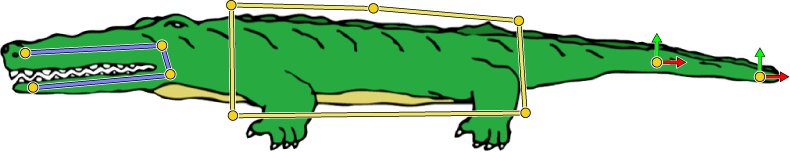
\includegraphics[scale=0.25]{alligator-avant}
  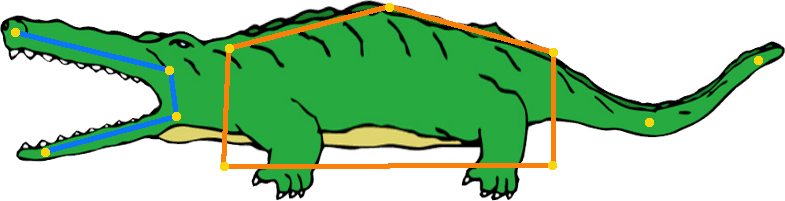
\includegraphics[scale=0.25]{alligator-apres}
  \caption{A gauche le modèle avant déformation et à droite le modèle
    après déplacement de certains points de contrôle}
  \label{INTall}
\end{figure}

Tout au long de ce travail, nos choix ont été motivés par la volonté
de fournir un outil permettant de déformer des points de l'espace de
manière interactive et fluide, et d'obtenir des formulations
mathématiques simples et claires. Le but de ce travail est de pouvoir
permettre à un utilisateur d'obtenir un outil de déformation
s'adaptant à ses besoins, en générant de façon automatique un outil
multidimensionnel de déformation, tout en lui laissant la possibilité
de paramétrer le comportement des différents outils utilisés.
%%% ----------------------------------------------------------------------


%%% Local Variables: 
%%% mode: latex
%%% TeX-master: "../thesis"
%%% End: 
